\documentclass{llncs}
\usepackage{url}
\usepackage{proof}
\usepackage{amssymb}
\usepackage{stmaryrd}
\usepackage{listings}
\usepackage{graphicx}
\usepackage{comment}

\newcommand{\dgm}[2][1.5]{
\begin{center}
\scalebox{#1}{
\includegraphics{diagrams/#2.pdf}
}
\end{center}
}

\newcommand{\todo}[1]{\textbf{TODO:} #1}
\newcommand{\jacques}[1]{\textsc{Jacques says:} #1}
\newcommand{\amr}[1]{\textsc{Amr says:} #1}
\newcommand{\roshan}[1]{\textsc{Roshan says:} 
  \textit{#1}
}

\hyphenation{a-reas}

%subcode-inline{bnf-inline} name Pi
%! swap+ = \mathit{swap}^+
%! swap* = \mathit{swap}^*
%! dagger =  ^{\dagger}
%! assocl+ = \mathit{assocl}^+
%! assocr+ = \mathit{assocr}^+
%! assocl* = \mathit{assocl}^*
%! assocr* = \mathit{assocr}^*
%! identr* = \mathit{uniti}
%! identl* = \mathit{unite}
%! dist = \mathit{distrib}
%! factor = \mathit{factor}
%! (o) = \fatsemi
%! (;) = \fatsemi
%! (*) = \times
%! (+) = +
%! foldB = fold_B
%! unfoldB = unfold_B
%! foldN = fold_N
%! unfoldN = unfold_N
%! trace+ = \mathit{trace}^{+}
%! trace* = \mathit{trace}^{\times}
%! :-* = \multimap
%! :-+ = \multimap^{+}
%! emptyset = \emptyset

%subcode-inline{bnf-inline} regex \{\{(((\}[^\}])|[^\}])*)\}\} name main include Pi
%! [^ = \ulcorner
%! ^] = \urcorner
%! [v = \llcorner
%! v] = \lrcorner
%! [[ = \llbracket
%! ]] = \rrbracket
%! ^^^ = ^{\dagger}
%! eta* = \eta
%! eps* = \epsilon
%! Union = \bigcup
%! in = \in
%! |-->* = \mapsto^{*}
%! |-->> = \mapsto_{\ggg}
%! |-->let = \mapsto_{let}
%! |--> = \mapsto
%! <--| = \mapsfrom
%! |- = \vdash
%! <=> = \Longleftrightarrow
%! <-> = \leftrightarrow
%! -> = \rightarrow
%! ~> = \leadsto
%! ::= = ::=
%! /= = \neq
%! vi = v_i
%! di = d_i
%! si = s_i
%! sj = s_j
%! F = \texttt{F}
%! T = \texttt{T}
%! forall = \forall
%! exists = \exists
%! empty = \emptyset
%! eta = \eta
%! where = \textbf{where}
%! epsilon = \varepsilon
%! least = \phi
%! loop+ = loop_{+}
%! loop* = loop_{\times}
%! CatC = {\mathcal C}
%! CatA = {\mathcal A}
%! gamma = \gamma
%! {[ = \{
%! ]} = \}
%! elem = \in
%! dagger = ^\dagger
%! alpha = \alpha
%! beta = \beta
%! rho = \rho
%! @@ = \mu
%! @ = \,@\,
%! Pow = \mathcal{P}
%! Pi = \Pi
%! PiT = \Pi^{o}
%! PiEE = \Pi^{\eta\epsilon}_{+}
%! PiT = \Pi^{o}
%! PiTF = \Pi^{/}
%! bullet = \bullet
%! * = \times

%%%%%%%%%%%%%%%%%%%%%%%%%%%%%%%%%%%%%%%%%%%%%%%%%%%%%%%%%%%%%%%%%%%%%%%%%%%%%

\begin{document}
\title{Fractional Types}
\author{Roshan P. James \and Zachary Sparks \and Jacques Carette \and Amr Sabry}
\institute{Indiana University and McMaster University}
\maketitle

%%%%%%%%%%%%%%%%%%%%%%%%%%%%%%%%%%%%%%%%%%%%%%%%%%%%%%%%%%%%%%%%%%%%%%%%%%%%%
\begin{abstract}
  In previous work, we developed a \emph{first-order},
  information-preserving, and reversible programming language {{Pi}} founded
  on type isomorphisms. Being restricted to first-order types limits the
  expressiveness of the language: it is not possible, for example, to
  abstract common program fragments into a higher-level combinator. In this
  paper, we introduce a higher-order extension of {{Pi}} based on the novel
  concept of \emph{fractional types} {{1/b}}. Intuitively, a value of a
  fractional type {{1/v}} represents \emph{negative} information. A
  higher-order function is modeled by a pair {{(1/v1,v2)}} with {{1/v1}}
  representing the needed argument and {{v2}} representing the
  result. Fractional values are first-class: they can be freely propagated
  and transformed but must ultimately --- in a complete program --- be offset
  by the corresponding amount of positive information.
\end{abstract}

%%%%%%%%%%%%%%%%%%%%%%%%%%%%%%%%%%%%%%%%%%%%%%%%%%%%%%%%%%%%%%%%%%%%%%%%%%%%%
\section{Introduction} 

We are witnessing a convergence of ideas from several distinct research
communities (physics, mathematics, and computer science) towards replacing
\emph{equalities} by \emph{isomorphisms}. The combined programme 
has sparked a huge amount of research that unveiled
new and surprising connections between geometry, algebra, logic, and
computation (see~\cite{baez2011physics} for an overview).

In the physics community, Landauer~\cite{Landauer:1961,Landauer},
Feynman~\cite{springerlink:10.1007/BF02650179}, and others have interpreted
the laws of physics as fundamentally related to computation. In more detail,
the great majority of the laws of physics are formulated as equalities
between different physical observables, such as Newton's second law of
classical mechanics ($F=\dot{p}$).
The insight of Landauer, Feynman, etc. is that
\emph{different} physical observables should not be related by an
\emph{equality} but more appropriately by an \emph{isomorphism} that
witnesses, explains, and models the process of transforming one observable to
the other.

In the mathematics and logic community, Martin-L\"of developed an extension
of the simply typed $\lambda$-calculus originally intended to provide a
rigorous framework for constructive
mathematics~\cite{citeulike:7374951}. This theory has been further extended
with \emph{identity types} representing the proposition that two terms are
``equal.'' (See~\cite{streicher,warren} for a survey.) Briefly speaking,
given two terms $a$ and $b$ of the same type $A$, one forms the type
$\texttt{Id}_A(a,b)$ representing the proposition that~$a$ and~$b$ are equal:
in other words, a term of type $\texttt{Id}_A(a,b)$ witnesses, explains, and
models the process of transforming $a$ to $b$ and vice-versa.

In the computer science community, the theory and practice of type
isomorphisms is well-established. Originally, such type isomorphisms were
motivated by the pragmatic concern of searching large libraries of functions
by providing one of the many possible isomorphic types for the desired
function~\cite{Rittri:1989:UTS:99370.99384}. More recently, type isomorphisms
have taken a more central role as \emph{the} fundamental computational
mechanism from which more conventional, i.e., irreversible computation, is
derived. In more detail, in our own previous
work~\cite{James:2012:IE:2103656.2103667,rc2011,rc2012} we started with the
notion of type isomorphism as the ``right'' starting point for a theory of
computation. The central technical contribution was the development of a
family of programming languages, {{Pi}} with various superscripts, in which
every computation is an isomorphism. Other major results are that all such
computations preserve the information-theoretic entropy, that the languages
are logically reversible, and that they have models in various flavors of
symmetric monoidal categories (which are the backbone of models for linear
logic and quantum computation). We have also invested a significant amount of
time in using {{Pi}} as an actual programming language and established
several idioms for programming large classes of interesting (recursive)
programs in {{Pi}}.

A major open problem remains, however: a higher-order extension of
{{Pi}}. This extension is of fundamental importance in all the originating
research areas. In physics, it allows a process or observer to be treated as
``data'' that can be transformed by higher-level processes or observed by
meta-level observers. In mathematics and logic, it allows the equivalence
between different proofs of type $\texttt{Id}_A(a,b)$ to itself be expressed
as an isomorphism (of a higher type)
$\texttt{Id}_{\texttt{Id}_A(a,b)}(p,q)$. Finally, in computer science,
higher-order types allow code to abstract over other code fragments as well
as the manipulation of code as data and data as code.

Technically speaking, obtaining a higher-order extension requires the
construction of a \emph{compact closed category} from the underlying monoidal
category for~{{Pi}}. Although the general idea of such a construction is
well-understood, the details of adapting it to an actual programming language
as subtle (as we explain in the main body of the paper).  Our main novel
technical device to achieving the higher-order extension is a
\emph{fractional type}, which we so named because of its duality with
conventional product types.  By adding a formal (linear) dual to (type
theoretic) products, we can internalize the notion that ``taking an input''
corresponds to negative information, which turns out to be the basis of
first-class functions. The remainder of the paper reviews {{Pi}} and then
introduces the syntax and semantics of the extension with fractional
types. We then study the properties of the extended language and establish
its expressiveness via several constructions and examples that exploit its
ability to model higher-order computations.

%% AMR:
%% \roshan{It is unclear what the Id types refer to. We should provide
%%   some more context here}
%% I think the previous paragraph in the intro that talks about Martin-Lof type 
%% theory provides the context. Anything else??

%%%%%%%%%%%%%%%%%%%%%%%%%%%%%%%%%%%%%%%%%%%%%%%%%%%%%%%%%%%%%%%%%%%%%%%%%%%%%
\section{Background: {{Pi}} }
\label{sec:pi}

We review our language {{Pi}} providing the necessary background and
context for our higher-order extension.\footnote{The presentation in this
  section focuses on the simplest version of {{Pi}}. Other versions
  include the empty type, recursive types, and trace operators but these
  extensions are orthogonal to the higher-order extension emphasized in this
  paper.} The terms of {{Pi}} are not classical values and functions;
rather, the terms are isomorphism witnesses.  In other words, the terms of
{{Pi}} are proofs that certain ``shapes of values'' are isomorphic.
And, in classical Curry-Howard fashion, our operational semantics shows how
these proofs can be directly interpreted as actions on ordinary values which
effect this shape transformation. Of course, ``shapes of values'' are very
familiar already: they are usually called \emph{types}.  But frequently one
designs a type system as a method of classifying terms, with the eventual
purpose to show that certain properties of well-typed terms hold, such as
safety.  Our approach is different: we start from a type system, and then
present a term language which naturally inhabits these types, along with an
appropriate operational semantics.

\paragraph*{Data.}
We view {{Pi}} as having two levels:  it has traditional values, given by:
%subcode{bnf} include main
% values, v ::= () | left v | right v | (v, v)
\noindent and these are classified by ordinary types:
%subcode{bnf} include main
% value types, b ::= 1 | b + b | b * b 
\noindent Types include the unit type {{1}}, sum types {{b1 + b2}}, and
products types {{b1*b2}}.  Values includes {{()}} which is the only value of
type {{1}}, {{left v}} and {{right v}} which inject {{v}} into a sum type,
and {{(v1,v2)}} which builds a value of product type. But these values should
be regarded as largely ancillary.  In particular we do not treat the above
values as first-class citizens.  They only occur when we want to observe the
effect of an isomorphism.

\paragraph*{Isomorphisms.} The important terms of {{Pi}} are witnesses to
(value) type isomorphisms.  They are also typed, by the shape of the (value)
type isomorphism they witness {{b <-> b}}.  Specifically, they are witnesses to
the following isomorphisms:
%subcode{bnf} include main
%! columnStyle = r@{\hspace{-0.5pt}}c@{\hspace{-0.5pt}}l
%swap+ :&  b1 + b2 <-> b2 + b1 &: swap+
%assocl+ :&  b1 + (b2 + b3) <-> (b1 + b2) + b3 &: assocr+
%identl* :&  1 * b <-> b &: identr*
%swap* :&  b1 * b2 <-> b2 * b1 &: swap*
%assocl* :&  b1 * (b2 * b3) <-> (b1 * b2) * b3 &: assocr*
%dist :&~ (b1 + b2) * b3 <-> (b1 * b3) + (b2 * b3)~ &: factor
\noindent Each line of the above table introduces a pair of dual
constants\footnote{where {{swap*}} and {{swap+}} are self-dual} that witness
the type isomorphism in the middle.  These are the base (non-reducible) terms
of the second, principal level of {{Pi}}. Note how the above has two
readings: first as a set of typing relations for a set of constants. Second,
if these axioms are seen as universally quantified, orientable statements,
they also induce transformations of the (traditional) values. The
(categorical) intuition here is that these axioms have computational content
because they witness isomorphisms rather than merely stating an extensional
equality.

The isomorphisms are extended to form a congruence relation by adding the
following constructors that witness equivalence and compatible closure:
%subcode{proof} include main
%@  ~
%@@ id : b <-> b 
%
%@ c : b1 <-> b2
%@@ sym c : b2 <-> b1
%
%@ c1 : b1 <-> b2
%@ c2 : b2 <-> b3
%@@ c1(;)c2 : b1 <-> b3
%---
%@ c1 : b1 <-> b3
%@ c2 : b2 <-> b4
%@@ c1 (+) c2 : b1 + b2 <-> b3 + b4
%
%@ c1 : b1 <-> b3
%@ c2 : b2 <-> b4
%@@ c1 (*) c2 : b1 * b2 <-> b3 * b4
\noindent The syntax is overloaded: we use the same symbol at the value-type level
and at the isomorphism-type level for denoting sums and products.  Hopefully
this will not cause undue confusion.

It is important to note that ``values'' and ``isomorphisms'' are completely
separate syntactic categories which do not intermix. The semantics of the
language come when these are made to interact at the ``top level'', a new
syntactic category:
%subcode{bnf} include main
% top level term, l ::= c v
\noindent We refer to this as \emph{application}.

% \noindent
% To summarize, the syntax of {{Pi}} is given as follows. 

% \begin{definition}{(Syntax of {{Pi}})}
% \label{def:Pi}
% %subcode{bnf} include main
% % value types, b ::= 1 | b+b | b*b 
% % values, v ::= () | left v | right v | (v,v) 
% %
% % iso.~types, t ::= b <-> b
% % base iso ::= swap+ | assocl+ | assocr+ 
% %     &|& unite | uniti | swap* | assocl* | assocr* 
% %     &|& dist | factor 
% % iso comb., c ::= iso | id | sym c | c (;) c | c (+) c | c (*) c 
% % top level term, l ::= c v
% \end{definition}

Mathematically, {{Pi}} can be interpreted in the category of finite sets and
bijections: each value type denotes a finite set of a size calculated by
viewing the types as natural numbers and each combinator {{c : b1 <-> b2}}
denotes a bijection between the sets denoted by~{{b1}}
and~{{b2}}. Operationally, the semantics of {{Pi}} is given using two
mutually recursive interpreters: one going forward and one going
backwards. The use of {{sym}} switches control from one evaluator to the
other. We will present the operational semantics in the next section along
with the extension with fractional types and values. For now, we state
without proof that the evaluation of well-typed combinators always terminates
and that {{Pi}} is logically reversible, i.e., that for all combinators 
{{c : b1 <-> b2}} and values {{v1 : b1}} and {{v2 : b2}} we have the forward
evaluation of {{c v1}} produces {{v2}} iff the backwards evaluation of 
{{c v2}} produces {{v1}}.

%% AMR:
%% \jacques{Since we have Agda code for the above, should we refer to it
%% here, and make it available?}
%% That is a great idea but it would take a significant amount of time to
%% clean up the code and make it presentable. If someone is willing to do
%% that, then we should definitely add a reference to the code and make it
%% available.
%% Jacques:  Right.  I'll definitely work on cleaning up the paper first,
%% then see if there is time left for the code.

The language presented above, at the type level, models a commutative ringoid
where the multiplicative structure forms a commutative monoid, but the
additive structure is just a commutative semigroup.  Note that the version of
{{Pi}} that include the empty type with its usual laws exactly captures, at
the type level, the notion of a \emph{semiring} (occasionally called a
\emph{rig}) where we replace equality by isomorphism.  This can also be also
compared to \emph{bimonoidal categories}.  As is usual with type theories,
the coherence conditions (pentagonal and triangle identity) are not explicit,
but would correspond to certain identity types being trivial.

%%%%%%%%%%%%%%%%%%%%%%%%%%%%%%%%%%%%%%%%%%%%%%%%%%%%%%%%%%%%%%%%%%%%%%%%%%%%
\section{The Language: {{PiTF}} }

The language {{Pi}} models isomorphisms of values rather well.  However,
purposefully, it has no distinguished notion of \emph{input} or
\emph{output}; more precisely, because of strict preservation of information,
these two concepts coincide.  This is the root of reversibility. But if we
want to model functions of any flavor as values, we need to differentiate
between these notions. We also clearly need to relax the strict separation
between values and isomorphisms as the notion of ``higher-order'' requires
that isomorphisms be represented as values. Our idea, inspired by
computational dualities~\cite{Filinski:1989:DCI:648332.755574,Curien:2000},
polarity~\cite{Girard87tcs,10.1109/LICS.2010.23}, and the categorical notion
of \emph{compact
  closure}~\cite{Selinger:2007:DCC:1229185.1229207,Abramsky:2004:CSQ:1018438.1021878},
is to introduce a \emph{formal dual} for our types.  We thus consider a type
in a negative position to possess negative information, as it is really a
request for information.  Since information is logarithmic, this means that a
request for information should behave like a \emph{fractional type}.

% \roshan{It is unclear how fractions help differentiate between inputs
%   and outputs. On first reading this seemed promising, but nothing
%   in the rest of the paper substantiates this point of view.}
% AMR: a function a -o b is modeled by (1/a,b) not (a,b) 
% Jacques: Exactly!  1/a is negative information is input, b is positive is
%    output.
%

% \roshan{I think we should arrive at relational programming as a means
%   of giving semantics to fractionals, rather than the other way
%   round. To show that relational programming is reversible, one does
%   not need to resort to fractionals. Everyone understand that
%   relations can be reversed and none of this setup with {{Pi}} is
%   required for that. Our key point should be to communicate that
%   fractionals have a clean semantics in the setting of relational
%   programming rather than the other way round.}
% AMR: relations are indeed only presented as a way to explain the semantics

The extension of the sets of types and values from {{Pi}} to {{PiTF}} is
simple:

%subcode{bnf} include main
% value types, b ::= ... | 1/b
% values, v ::= ... | 1/v

For a given type {{b}}, the values of type {{1/b}} are of the form {{1/v}}
where {{v : b}}. Note that {{1/v}} is purely formal, as is {{1/b}}. We have
however some informal intuition about the \emph{meaning} of such fractional
types and values. (See Sec.~\ref{sec:cat} for more discussion about this
point.) In more detail, given a symmetric monoidal category modeling a
certain language (like {{Pi}}), one can obtain a higher-order extension of
the language by extending the category to a \emph{compact closed} one, i.e.,
a category in which morphisms are representable as objects. The key to this
extension is to add dual objects (in our case the fractionals) satisfying the
following isomorphism witnessed by two new combinators {{eta*_b}} and
{{eps*_b}}:

{{eta*_b : 1 <-> 1/b * b : eps*_b}}

\noindent From a programming perspective, we think of a value {{1/v}} as a
\emph{first-class constraint} that can only be satisfied if it is matched
with an actual value {{v}} or as a \emph{pattern} representing the absence of
some information of a specific shape (i.e., \emph{negative information}),
that can only be reconciliated by an actual value {{v}}. The combinator
{{eta*_b : 1 <-> 1/b * b}} thus represents a fission point which creates ---
out of no information --- an equal amount of negative and positive
information. Symmetrically, the combinator {{eps*_b : 1/b * b <-> 1}} matches
up an equal amount of negative and positive information producing no residual
information. 

From the categorical perspective, versions of compact closed categories were
introduced by Abramsky and Coecke~\cite{Abramsky:2004:CSQ:1018438.1021878}
and by Selinger~\cite{Selinger:2007:DCC:1229185.1229207} as the
generalization of monoidal categories to model quantum computation.  The
first and most intuitive example of such categories is the category of finite
sets and relations. In that case, the dual operation (i.e., the fractional
type) collapses by defining {{1/b}} to be {{b}}. In spite of this degenerate
interpretation of fractionals, this is still an interesting category as it
provides a model for a reversible higher-order language. Indeed, any relation
is trivially reversible and any relation between {{b1}} and {{b2}} can be
represented as a subset of {{b1 * b2}}, i.e., as a value. A more interesting
example is the category of finite dimensional vector spaces and linear maps
(or even the category of finite dimensional Hilbert spaces). In such
categories the dual operation takes a vector space (consisting of ``column
vectors'') to the dual vector space (consisting of ``row vectors''). These
vector spaces are isomorphic, but they are nevertheless quite different,
being $(1,0)$ and $(0,1)$ tensors (respectively).  In other words, the
category provides a more refined model in which isomorphic
negative-information values and positive-information are not identified.

In this section, we provide a simple semantics of {{PiTF}} in the category of
finite sets and relations. In other words, we interpret each combinator {{c :
    b1 <-> b2}} as a \emph{relation} between the sets denoted by {{b1}} and
{{b2}} respectively. As we illustrate, this semantics allows \emph{arbitrary}
relations (including the empty relation and relations that are not
isomorphisms) to be represented as values in {{PiTF}}.  In Sec.~\ref{sec:cat}
we discuss more refined semantics that are more suitable for richer
categories.

\begin{definition}[Denotation of Value Types {{ [[ b ]] }}]
\label{chx:def:denot}
Each type denotes a finite set of values as follows:
%subcode{opsem} include main
%! <- = \leftarrow
%! union = \cup
% [[1]] '= {[ () ]}
% [[b1 + b2]] '= {[ left v ~|~ v <- [[b1]] ]} union {[ right v ~|~ v <- [[b2]] ]}
% [[b1 * b2]] '= {[ (v1, v2) ~|~ v1 <- [[b1]], v2 <- [[b2]] ]}
% [[1/b]] '= {[ 1/v ~|~ v <- [[b]] ]}
\end{definition}

The denotation of combinators as relations is given below. We specify
relations using a deductive system whose judgments are of the form 
{{ v1 ~~c~~ v2 }} indicating that the pair {{(v1,v2)}} is in the relation 
denoted by {{c}}.

\begin{definition}[Relational semantics]
\label{def:relational-PiTF}
Each combinator {{c : b1 <-> b2}} in {{PiTF}} denotes a relation
as specified below. 
%subcode{proof} include main
%@ ~
%@@ (left v) ~~swap+~~ (right v)
%
%@ ~
%@@ (right v) ~~swap+~~ (left v)
%----
%@ ~
%@@ (left v) ~~assocl+~~ (left (left v))
%
%@ ~
%@@ (right (left v)) ~~assocl+~~ (left (right v))
%----
%@ ~
%@@ (right (right v)) ~~assocl+~~ (right v)
%
%@ ~
%@@ (left (left v)) ~~assocr+~~ (left v)
%----
%@ ~
%@@ (left (right v)) ~~assocr+~~ (right (left v))
%
%@ ~
%@@ (right v) ~~assocr+~~ (right (right v))
%----
%@ ~
%@@ ((), v) ~~unite~~ v
%
%@ ~
%@@ v ~~uniti~~ ((), v)
%----
%@ ~
%@@ (v1, v2) ~~swap*~~ (v2, v1)
%----
%@ ~
%@@ (v1, (v2, v3)) ~~assocl*~~ ((v1, v2), v3)
%
%@ ~
%@@ ((v1, v2), v3) ~~assocr*~~ (v1, (v2, v3))
%----
%@ ~
%@@ (left v1, v3) ~~dist~~ (left (v1, v3))
%
%@ ~
%@@ (right v2, v3) ~~dist~~ (right (v2, v3))
%----
%@ ~
%@@ (left (v1, v3)) ~~factor~~ (left v1, v3)
%
%@ ~
%@@ (right (v2, v3)) ~~factor~~ (right v2, v3)
%----
%@ ~
%@@ v ~~id~~ v
%
%@ v' ~~c~~ v
%@@ v ~~(sym c)~~ v'
%
%@ v1 ~~c1~~ v2
%@ v2 ~~c2~~ v3
%@@ v1 ~~(c1(;)c2)~~ v3
%----
%@ v ~~c1~~ v'
%@@ (left v) ~~(c1 (+) c2)~~ (left v')
%
%@ v ~~c2~~ v'
%@@ (right v) ~~(c1 (+) c2)~~ (right v')
%----
%@ v1 ~~c1~~ v1'
%@ v2 ~~c2~~ v2'
%@@ (v1, v2) ~~(c1 (*) c2)~~ (v1', v2')
%----
%@ ~
%@@ () ~~eta*_b~~ (1/v,v)
%
%@ ~
%@@ (1/v,v) ~~eps*_b~~ ()
\end{definition}

\begin{multicols}{2}
  \dgm{eta_times2}

  \dgm{eps_times2}  
\end{multicols}

The operational semantics define a relation rather than a function, but the
goal is for them to still be reversible; in particular, we wish for the
relation to mode check so that for any combinator {{c}} we can treat either
its left or its right side as an input; this allows us to define {{sym}} as
just an argument swap. We can then give an operational interpretation to the
semantic relation by defining two functions: a forward evaluator and a
backwards evaluator that exercise the relation in opposite directions. It is
straightforward to check that if the forward evaluation of {{c v1}} produces
{{v2}} as a possible answer then the backwards evaluation of {{c v2}}
produces {{v1}} as a possible answer.

In the interest of brevity, we have treated the type annotations in the base
isomorphisms as implicit; for example, the rule for {{assocr*}} should really
read:

%subcode{proof} include main
%@ v1 in b1
%@ v2 in b2
%@ v3 in b3
%@@ ((v1, v2), v3) ~~assocr*_{b1, b2, b3}~~ (v1, (v2, v3))

% \roshan{ In the rules above it is unclear as to which v is chosen in
%   the rule for eta. It is unclear that these rules are logically
%   reversible.  }

% \begin{proposition}[Logical Reversibility]
% \label{chx:prop:logrev-tracep}
% For all combinators {{c : b1 <-> b2}} and values {{v1 : b1}} and 
% {{v2 : b2}} we have {{v1 ~~c~~ v2}} iff {{v2 ~~(sym c)~~ v1}}.
% \end{proposition}

% Some thoughts on a relational semantics. We define {{ a <-> b }}
% $\equiv$ {{a R b}}

% \noindent
% We now have primitives:
% %subcode{opsem} include main
% % swap*:b1*b2<->b2*b1 '= {[ ((v1, v2), (v2, v1)) ~|~ v1 in b1, v2 in b2 ]}
% % swap+:b1+b2<->b2+b1 '= {[ ((left v1), (right v1)) and ((right v2), (left v2)) 
% %                     && ~~~| v1 in b1, v2 in b2]}
% % assocl*:b1*(b2*b3)<->(b1*b2)*b3 '= {[ ((v1, (v2, v3)), ((v1, v2), v3)) 
% %                   & & ~~~|~ v1 in b1, v2 in b2, v3 in b3]}
% etc..

% \noindent
% closure combinators:
% %subcode{opsem} include main
% % sym c '= {[(v2, v1) ~|~ (v1, v2) in c ]}
% % c1 (;) c2 '= {[(v1, v3) ~|~ v2 in b2, (v1, v2) in c1, (v2, v3) in c2 ]}
% % c1 (*) c2 '= {[((v1, v2), (v3, v4)) ~|~ (v1, v3) in c1, (v2, v4) in c2 ]}
% etc..

% \noindent
% Now we have 
% %subcode{opsem} include main
% % eta* '= {[ ((), (v, 1/v)) ~|~ v in b ]}
% % eps* '= {[ ((v, 1/v), ()) ~|~ v in b ]}

% Now {{PiTF}} is logically reversible in that for all {{c:b1<->b2}} we
% have {{c^{dagger}: b2 <-> b1}} such that 
% %
% {{c^{dagger} = {[(v2, v1)~|~(v1,v2) in c ]} }}. This is
% straightforward from the definitions above. 

% I think defining eval is an open problem.  Consider a few relations:

% \begin{enumerate}
% \item 
% {{empty = {[ ]} }}

% \item 
% {{full =  {[ R, G, B ]} * {[ R, G, B ]} }}

% \item 
% {{id  =  {[ (R, R), (G, G), (B, B) ]} }}

% \item 
% {{cycle = {[ (R, R), (R, G), (G, G), (G, B), (B, B), (B, R) ]} }}
% \end{enumerate}
 
% Can we define an {{eval}} that meaningfully distinguishes these? What
% can we say about {{(c (;) c^^^) v}} based on {{eval}}?  Here are
% several possible {{eval}} definitions:

% \begin{enumerate}
% \item {{ c v = v'}} where {{ v' in {[ v' ~|~ (v, v') in c ]} }}. The
%   eval maps {{b1 -> b2}}. 

% \item {{ c v = {[ v' ~|~ (v, v') in c ]} }}. The eval maps {{b1 -> Pow(b2)}}.

% \item {{ c vs = {[ v' ~|~ (v, v') in c, v in vs ]} }}. where
%   {{vs:Pow(b1)}}. The eval maps {{Pow(b1) -> Pow(b2)}}. 

% \end{enumerate}

% For the relations above, none of the suggested eval definitions give a
% logically reversible semantics.

% \roshan{If {{|b1|=|b2|}}, can we define all relations between {{b1}} and
% {{b2}}? If yes, then we have a model for {{PiTF}} where the objects
% are sets {{b}} and the morphisms are the relations between objects of
% equal size.}

% \roshan{ I suspect that all relations can be constructed, but we have
%   to show this. This is not obvious.}

% \roshan{In the judgments below it is misleading that only {{eta*}}
%   appears indexed by a type. To construct each family of relations,
%   the corresponding definition must be indexed by their types. In
%   other words, there is nothing special about {{eta*}}. Further, I am
%   unsure of how to format this so that the combinators are correctly
%   indexed by their types for both primitives and for composition
%   combinators. We could do the following, but it seems to be a
%   overkill.}

% %subcode{proof} include main
% %@ v1 in [[b1]]
% %@ v2 in [[b2]]
% %@ v3 in [[b3]]
% %@@ (v1, (v2, v3)) ~assocl*~ ((v1, v2), v3)

%%%%%%%%%%%%%%%%%%%%%%%%%%%%%%%%%%%%%%%%%%%%%%%%%%%%%%%%%%%%%%%%%%%%%%%%%%%%
\section{Expressiveness and Examples} 

In the following, we use {{bool}} as an abbreviation of {{1+1}} 
with {{true}} as an abbreviation for {{left ()}} and {{false}} as an 
abbreviation for {{right ()}}.


%%%%%%%%%%%%
\subsection{First-Class Relations}

As motivated, with fractional types, we can define a value that denotes a
first-class function or relation. Indeed a value of type {{1/b1 * b2}} is a
pair of a \emph{constraint} that can only be satisfied by some {{v1 : b1}}
and a value {{v2 : b2}}. In other words, it corresponds to a function or
relation which when ``given'' a value {{v1 : b1}} ``releases'' the value 
{{v2 : b2}}. To emphasize this view, we introduce the abbreviation:

%subcode{bnf} include main
%  b1 :-* b2 &::=& 1/b1 * b2

\begin{multicols}{2}
  \dgm{function-times}

  \dgm{delimc-times}
\end{multicols}

\noindent which suggests a function-like behavior for the pair of a fractional value
and a regular value. What is remarkable is that we can almost trivially turn
any combinator {{c : b1 <-> b2}} into a (constant) value of 
type {{b1 :-* b2}} as shown below:

%subcode{opsem} include main
%! columnStyle = rcl
% name &:& (b1 <-> b2) -> (1 <-> (b1 :-* b2))
% name c &=& eta*_{b1} (;) (id (*) c)

As a simple example, consider the combinator {{swap+}} denoting boolean
negation.  It is straightforward to check that the combinator 
{{name swap+ : 1 <-> (bool :-* bool)}} denotes the following relation:

%subcode{proof} include main
%@ ~
%@@ () ~~(name swap+)~~ (1/false,true)
%
%@ ~
%@@ () ~~(name swap+)~~ (1/true,false)

\noindent The relation {{name swap+}} maps {{()}} to a value which can be used
to convert any {{false}} to {{true}} and vice-versa. We formalize this
``apply'' combinator below.

%%%%%%%%%%%%
\subsection{Higher-Order Relations}

We are now a small step from implementing various higher-order
combinators that manipulate functions or relations. In particular, we
can \emph{apply} and \emph{compose} values representing relations as
shown below:

%subcode{opsem} include main
%! columnStyle = rcl
% apply &:& (b1 :-* b2) * b1 <-> b2
% apply &=& swap* (;) assocl* (;) (swap* (*) id) (;) (eps*_{b1} (*) id) (;) unite

\begin{multicols}{2}
  \dgm[1.2]{apply-times1}

  \dgm{apply-times2}
\end{multicols}


\noindent At the type level, the computation proceeds as follows:
%subcode{bnf} include main
%  (b1 :-* b2) * b1 &=& (1/b1 * b2) * b1 & 
%     &<->& b1 * (1/b1 * b2) & (swap*)
%     &<->& (b1 * 1/b1) * b2) & (assocl*)
%     &<->& (1/b1 * b1) * b2) & (swap* (*) id)
%     &<->& 1 * b2 & (eps*_{b1} (*) id)
%     &<->& b2 & (unite)

\noindent Intuitively, we simply match the incoming argument of type {{b1}} with
the constraint encoded by the function. If they match, they cancel
each other and the value of type {{b2}} is exposed with no
constraints. Otherwise, the result is undefined.

\noindent A flipped variant is also useful:
%subcode{opsem} include main
%! columnStyle = rcl
% apply' &:& b1 * (b1 :-* b2) <-> b2
% apply' &=& assocl* (;) (swap* (*) id) (;) (eps*_{b1} (*) id) (;) unite

\noindent Function or relation composition is now straightforward:

%subcode{opsem} include main
%! columnStyle = rcl
% compose &:& (b1 :-* b2) * (b2 :-* b3) -> (b1 :-* b3)
% compose &=& assocr* (;) (id (*) apply')

\begin{multicols}{2}
  \dgm[1.0]{compose-times1}

  \dgm{compose-times2}
\end{multicols}

\dgm{compose-times3}


\noindent Again, at the type level, the computation proceeds as follows:

%subcode{bnf} include main
%  (b1 :-* b2) * (b2 :-* b3) &=& (1/b1 * b2) * (1/b2 * b3) & 
%     &<->& (1/b1 * (b2 * (1/b2 * b3)) & (assocr*)
%     &<->& (1/b1 * b3) & (id * apply')
%     &=& b1 :-* b3

%%%%%%%%%%%%
\subsection{Duality}

The final remarkable property of fractional types is that they
are involutive.  In particular, we have:

%subcode{opsem} include main
%! columnStyle = rcl
% doubleDiv &:& b <-> 1/(1/b)
% doubleDiv &=& uniti (;) (eta*_{1/b} (*) id) (;) assocr* (;) (id (*) eps*_b) (;) swap* (;) unite

\noindent At the type level, this computation proceeds as follows:

%subcode{bnf} include main
%  b &<->& (1 * b) & (uniti)
%    &<->& (1/(1/b) * 1/b) * b & (eta*_{1/b} (*) id)
%    &<->& 1/(1/b) * (1/b * b) & (assocr*)
%    &<->& 1/(1/b) * 1 & (id (*) eps*_b)
%    &<->& 1 * 1/(1/b) & (swap*)
%    &<->& 1/(1/b) & (unite)

%%%%%%%%%%%%
\subsection{Feedback, Iteration, and Trace Operators}

Mathematically speaking, recursion and iteration can be expressed using
categorical trace
operators~\cite{joyal1996traced,Hasegawa:1997:RCS:645893.671607}.  In a
language like {{Pi}} there are two natural families of trace operators
that can be defined, an additive family (explored in detail in our previous
work~\cite{rc2011}) and a multiplicative family (which is the focus of this
section).

In this case, we are given a computation {{c:b1 * b2 <-> b1 * b3}} and we
want to cancel the common type {{b1}}, to produce a new combinator
{{trace*~c:b2<->b3}}. For the evaluation of such a combinator, we are only
given a value {{v2 : b2}}. But to evaluate {{c}}, we must provide a pair
consisting of ``some'' value {{v1 : b1}} together with the given {{v2 : b2}}.
The needed value {{v1 : b1}} cannot be arbitrary: it must be such that is
is the value produced as the first component of the result.  In general, there
may be several such fixed-point values or none.  A few examples should help
explain the subtleties.

\begin{example}
Consider the combinator

{{c : bool * 1 <-> bool * 1}} 

{{c = id}}

\noindent Using {{trace*}}, we construct the
combinator {{trace* c : 1 <-> 1}}. Applying this to 
{{() : 1}} requires us to find a value {{b : bool}} such that 
{{(b,()) ~~c~~ (b,())}}. Given that {{c}} is the identity and that the type {{bool}} 
has two values, there are two values {{false}} and {{true}} that satisfy the 
constraint. In other words, expect that {{() ~~(trace* c)~~() }}.
\end{example}

\begin{example}
\label{ch3:ex:annihilate}
Consider a small variation on the combinator {{c}} above:

{{c : bool * 1 <-> bool * 1}} 

{{c = swap+ (*) id }}

\noindent which negates the boolean component of its incoming
pair. Using the multiplicative trace operator, we can construct the
combinator {{trace* c : 1 <-> 1}} as before. But now, applying this
combinator to {{() : 1}} requires us to find a value {{b : bool}} such
that {{(b,()) ~~c~~ (b,())}} which is impossible since {{c}} negates
{{b}}, i.e. {{c}} has no fixed points. Operationally, the evaluation of
such a combinator should produce no value (if it even terminates).
\end{example}

With fractionals, the multiplicative trace operator becomes expressible:

%subcode{opsem} include main
%! columnStyle = rcl
% trace*_b &:& ((b * b1) <-> (b * b2)) -> (b1 <-> b2)
% trace*_b c &=& uniti (;) (eta*_b (*) id) (;) assocr* (;) 
%            && (id (*) c) (;) assocl* (;) (eps*_b (*) id) (;) unite

Let's use the semantics to calculate the result of applying
{{trace*_{bool} (not (*) id)}} to {{false}}. We start
with the set {{ {[ false ]} }} which gets transformed as follows:
%subcode{opsem} include main
%! columnStyle = ll
% {[ ((),false) ]}  & (uniti)
% {[ ((1/false,false),false), ((1/true,true),false) ]} & (eta*_{bool} * id)
% {[ (1/false, (false,false)), (1/true,(true,false)) ]} & (assocr*)
% {[ (1/false, (true,false)), (1/true,(false,false)) ]} & (id (*) not )
% {[ ((1/false,true),false), ((1/true,false),false) ]} & (assocl*)
% emptyset & (eps*_{bool} * id)

%% \jacques{in the current paper, this seems to no longer make sense}
%% Yes I know, but I think we should leave it to explain the problem in Sec. 5
%% and motivate the different semantics

\begin{example}[Annihilation]
\label{ch3:ex;annihilation}
Consider the circuit below:
\dgm{not_trace}
As motivated earlier, it is clearly impossible for the constraint implied by
{{trace*}} to be satisfied as a boolean value {{v}} can never be the same as
its negation. Thus there is no incoming value of type {{b}} that can ever go
through the circuit. Indeed, if we call the circuit above {{c}}, then we can
calculate that {{c}} does not relate {{v}} to anything. We call such a
circuit an annihilation circuit.
\end{example}

%%%%%%%%%%%%%%%%%%%%%%%%%
\subsection{(Finite) Relational Programming}
\label{ch3:sec:lp}

Relational programming leverages set-theoretic relations and their
composition to express computational tasks in a declarative way. 
% For instance, consider this example:
% {{parent = {[ (A,B), (B,C), (A,D) ]} }}
% {{grandparent = parent (o) parent}}
% \noindent The example defines a relation {{parent}} specified using a
% set of tuples and another relation {{grandparent}} specified using the
% composition of two parent relations. If we wrote this example in a
% relational language (e.g., Prolog) and we executed the query
% {{grandparent(A)}}, we would get the answer {{ {[C]} }}.
It turns out that with the addition of the multiplicative trace, and
the move to relations motivated in the previous section, we can
express relational programming. We illustrate the idea using a
complete example. 

Consider the relation {{R}} on booleans given by:

{{ {[(false,false), (false,true), (true,false) ]}. }}

We show how to define a combinator {{c_R}} whose semantics is such that:

%subcode{proof} include main
%@ ~
%@@ false ~~c_R~~ false
%
%@ ~
%@@ false ~~c_R~~ true
%
%@ ~
%@@ true ~~c_R~~ false

The key idea is to find a combinator {{cInner : (a * bool) <-> (a * bool)}}
for some type {{a}} such that {{trace* cInner}} is the desired combinator
{{c_R}}.  A little experimentation shows that we get the desired behavior if
as follows:
% %subcode{proof} include main
% %@ ~
% %@@ ((false,false),false) ~~cInner~~ ((false,false),false) 
% %----
% %@ ~
% %@@ ((false,true),false) ~~cInner~~ ((false,true),true) 
% %----
% %@ ~
% %@@  ((false,true),true) ~~cInner~~ ((false,true),false) 
% %----
% %@ ~
% %@@ ((false,false),true) ~~cInner~~ ((true,false),true) 
% %----
% %@ ~
% %@@ ((true,false),false) ~~cInner~~ ((true,true),false)  
% %----
% %@ ~
% %@@ ((true,false),true) ~~cInner~~ ((true,true),true)  
% %----
% %@ ~
% %@@ ((true,true),false) ~~cInner~~ ((true,false),false) 
% %----
% %@ ~
% %@@ ((true,true),true) ~~cInner~~ ((false,false),true) 
% In the first three lines, the first argument is a fixed point and hence the
% multiplicative trace would map the second input to the second output
% producing the desired relation. In the remaining five cases, the first
% argument is not a fixed point and hence all these cases would be rejected as
% solutions to the constraint imposed by the multiplicative trace. It simply
% remains to find the actual realization of {{cInner}} that would produce the
% behavior above. 

%subcode{opsem} include main
%! columnStyle = rcl
% cInner &:& (bool * bool) * bool <-> (bool * bool) * bool
% cInner &=& sym (swap* (;) assocl* (;) (cnot (*) id) (;) assoct* (;) swap* (;) 
%        &&  toffoli (;) ((swap* (;) cnot (;) swap*) (*) id) (;)
%        &&  toffoli (;) (assocr* (;) swap* (;) toffoli (;) swap* (;) assocl*) (;)
%        &&  toffoli (;) (cnot (*) id))
%     
% c_R &:& bool <-> bool
% c_R &=& trace* cInner

% The above example should convince the reader that the language {{Pi}}
% with multiplicative trace is expressive enough to model finite relational
% programming. 
% %%%%%%%%%%%%%%%
% \subsection{Solving Constraints}
% \label{ch3:sec:constraints}

% A large class of constraint satisfaction problems can be expressed
% using multiplicative traces. We illustrate the main ideas with the
% implementation of a SAT solver.

% In the usual setting, an instance of SAT is a function~{{f}} which,
% when given some boolean inputs, returns {{true}} or {{false}}. The
% function returns {{true}} when the inputs satisfy the constraints
% imposed by the structure of {{f}} and a solution to the SAT problem is
% the set of all inputs on which {{f}} produces {{true}}. The basic idea
% of our construction is to generalize the annihilation circuit from
% Ex.~\ref{ch3:ex;annihilation} to only annihilate values that fail to
% satisfy the constraints represented by the SAT instance {{f}}. To
% achieve this goal, we must however deal with several important
% details.

% First, because we are in a reversible world, our instance of SAT must be
% expressed as an isomorphism: this is easily achieved by the construction
% which embeds any boolean function {{f}} into a reversible one {{iso_f}} with
% a larger domain and range.  Given such a reversible function {{iso_f}} which
% represents a SAT instance, we first construct the circuit below:

% \begin{center}
% \scalebox{1.2}{
%   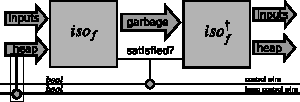
\includegraphics{diagrams/sat2.pdf}
% }
% \end{center}  

% As shown in the circuit, the reversible SAT instance {{iso_f}} takes
% two sets of values and produces two outputs. The incoming values
% labeled \textsf{inputs} are the inputs we need to test for
% satisfiability. The other incoming values labeled \textsf{heap} are
% the additional inputs needed to embed the original SAT instance {{f}}
% into a reversible function. If these \textsf{heap} values are all
% initialized to {{false}}, the output wire \textsf{satisfied?}
% corresponds to the output that {{f}} would have produced on
% \textsf{inputs}. The other outputs labeled \textsf{garbage} are not
% needed for their own sake but they are important because they are used
% as inputs to the adjoint of {{iso_f}} to reproduce the inputs exactly,
% in anticipation of closing the loop with {{trace*}}.

% To summarize, the top half of the circuit is the identity function
% except that we have also managed to produce a boolean wire labeled
% \textsf{satisfied?} that tells us if the inputs satisfy the desired
% constraints. We can take this boolean value and use it to decide
% whether to negate the bottom wire (labeled \textsf{control
%   wire}). Specifically, if the inputs do \emph{not} satisfy {{f}}, the
% control wire is negated. The last wire labeled \textsf{heap control
%   wire} is negated if the heap values do not have the right initial
% values, i.e., are not all {{false}}.

% Let us call the above construction {{sat_f}}. If we now close the loop
% using {{trace*}}, two things should happen:
% \begin{itemize}
% \item configurations in which the \textsf{heap} values are not all
%   {{false}} will be annihilated;
% \item configurations in which the \textsf{inputs} do not satisfy {{f}}
%   will cause the \textsf{satisfied?} wire to be negated and hence will
%   also be annihilated.
% \end{itemize}
% In other words, the only configurations that will survive are the ones in
% which the \textsf{inputs} satisfy {{f}}. We simply need to arrange to
% \emph{clone} these values and produce them as the output of the whole
% circuit. The final construction is therefore:

% \begin{center}
% \scalebox{1.5}{
%   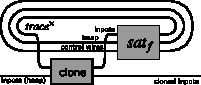
\includegraphics{diagrams/sat3.pdf}
% }
% \end{center}  

% To make the previous discussion concrete, we present a small, but
% complete, example. In our example, the SAT instance {{f}} is tiny: it
% takes two inputs. This function is embedded into a reversible function
% {{iso_f}} of type 
% {{((bool * bool) * bool) <-> ((bool * bool) * bool)}} where the last
% input represents the heap and the first two outputs represent the garbage. 
% The realization of {{sat_f}} given below is parametrized by such 
% a function {{iso_f}}. The inputs to {{sat_f}} are 
% \textsf{heap control}, \textsf{control}, \textsf{heap}, \textsf{input-1}, and 
% \textsf{input-2}. Its operation is simple: if the \textsf{heap} is {{true}}, 
% \textsf{heap control} is negated, and if the last output of {{iso_f}} 
% is {{false}}, \textsf{control} is negated:

% %subcode{opsem} include main
% %! columnStyle = rcl
% % sat_f &:& ((((bool * bool) * bool) * bool) * bool) <-> ((((bool * bool) * bool) * bool) * bool)
% % sat_f &=& ((swap* (*) id) (*) id) (;) 
% % && ((assocl* (*) id) (*) id) (;) 
% % &&   (((cnot (*) id) (*) id) (*) id) (;) 
% % &&   assocr* (;) 
% % &&   (assocr* (*) id) (;) 
% % &&   (swap* (*) id) (;) 
% % &&   assocr* (;) 
% % &&   (id (*) assocl*) (;) 
% % &&   (id (*) isof) (;) 
% % &&   swap* (;) 
% % &&   assocr* (;) 
% % &&   (id (*) (id (*) swap*)) (;) 
% % &&   (id (*) assocl*) (;) 
% % &&   (id (*) ((inot (*) id) (*) id)) (;)
% % &&   (id (*) (cnot (*) id)) (;) 
% % &&   (id (*) ((inot (*) id) (*) id)) (;)
% % &&   (id (*) assocr*) (;) 
% % &&   (id (*) (id (*) swap*)) (;) 
% % &&   assocl* (;)
% % &&   swap* (;)
% % &&   (id (*) Sym isof) (;) 
% % &&   (id (*) assocr*) (;) 
% % &&   assocl* (;) 
% % &&   assocl* 

% Given the construction of {{sat_f}} we can build the full solver as
% follows. The overall input is the cloning heap. The combinator given
% to {{trace*}} takes the cloning heap and the inputs flowing around the
% loop and produces two copies of these inputs. One copy is produced as
% the overall output and another is fed back around the loop. 

% %subcode{opsem} include main
% %! columnStyle = rcl
% % solve_f &:& bool * bool <-> bool * Bool
% % solve_f &=& trace* (
% % && (assocr* (*) id) (;) 
% % && assocr* (;)
% % && (id (*) swap*) (;)
% % && assocl* (;)
% % && (assocr* (*) id) (;)
% % && (clone2 (*) id) (;)
% % && swap* (;)
% % && (swap* (*) id) (;)
% % && ((swap* (*) id) (*) id) (;)
% % && assocl* (;)
% % && assocl* (;)
% % && (sat_f (*) id) (;)
% % && (assocr* (*) id) (;)
% % && (swap* (*) id) (;) 
% % && ((id (*) swap*) (*) id) (;)
% % && (assocl* (*) id) (;)
% % && ((id (*) swap*) (*) id))

% We can test our {{solve_f}} combinator using several SAT
% instances. Here are two possible instances. The first instance is
% satisfied by {{(false,false)}} and the
% second is satisfied by {{(false,true)}} and {{(true,true)}}.

% %subcode{opsem} include main
% %! columnStyle = rcl
% % iso_{f_1} &:& ((bool * bool) * bool) <-> ((bool * bool) * bool)
% % iso_{f_1} &=& (assocr* (;) swap* (;) toffoli (;) swap* (;) assocl*) (;)
% % && (((swap+ (*) id) (*) id) (;) toffoli (;) ((swap+ (*) id) (*) id)) (;) 
% % && (id (*) swap+)
% % 
% % iso_{f_2} &:& ((bool * bool) * bool) <-> ((bool * bool) * bool)
% % iso_{f_2} &=& toffoli

% It can indeed be verified using the semantics that the {{solve_f}}
% combinators instantiated with the SAT instances produce the expected
% results. 

%%%%%%%%%%%%%%%%%%%%%%%%%%%%%%%%%%%%%%%%%%%%%%%%%%%%%%%%%%%%%%%%%%%%%%%%%%%%%
\section{Discussion}
\label{sec:cat} 

The interpretation of {{PiTF}} in the category of sets and relations is
adequate in the sense that it produces a language in which every program is a
reversible relation and in which relations are first-class values. This
relational model is however, unsatisfactory, for several reasons:

\begin{itemize}
\item the type {{1/b}} is interpreted in the same way as {{b}} which gives no
  insight into the ``true meaning'' of fractionals;
\item the interpretation is inconsistent with the view of types as algebraic
  structures; for example, {{Pi}} with the empty type, is the
  categorificationi of a semiring but although fractional types in {{PiTF}}
  syntactically ``look like'' rational numbers, there is no such formal
  connection to the rational numbers;
\item finally, we have lost some delicate structure moving from {{Pi}} to
  {{PiTF}} as we can express arbitrary relations between types and not just
  isomorphisms.
\end{itemize}

For these reasons, it is interesting to consider other possible semantic
interpretations of fractionals. A natural alternative is to use the
``canonical'' compact closed category, that is finite dimensional vector
spaces and linear maps. We outline the main features of such an
interpretation:

\begin{itemize}
\item before we talk about vector spaces, we must fix an underlying
  field. For simplicity in the following discussion we choose the underlying
  field to be the field of booleans with two elements labeled \texttt{F} and
  \texttt{T}
\item each type {{b}} in {{PiTF}} is interpreted as a finite dimensional
  vector space $\mathbf{V}_b$ over the field of booleans. Of particular
  interest:
  \begin{itemize}
  \item every vector space contains a zero vector which means that the type
    {{0}} (if included in {{PiTF}} would not be the ``empty'' type --- it
    would contain the empty vector. Furthermore all combinators would be
    partial as they would have to map the zero vector to itself. 
  \item the type {{1}} is interpreted as a 1-dimensional vector space and hence
    is isomorphic to the underlying field.
  \item the fractional type {{1/b}} is interpreted as the dual vector space
    of the vector space $\mathbf{V}_b$ representing {{b}} consisting of all
    the \emph{linear functionals} on $\mathbf{V}_b$.
  \item one can then validate certain desirable properties: {{1/(1/b)}} is
    isomorphic to {{b}}; and {{eps*_b}} corresponds to a bilinear form which
    maps a dual vector and a vector to a field element.
  \end{itemize}
\end{itemize}

Although this semantics appears to have ``better'' properties than the
relational one, we argue that it is not \emph{the} ``perfect'' semantics. By
including the zero vector, the language has again additional partial
morphisms that do not correspond to isomorphisms and it is difficult to
reconcile the interpretation with the view that the types are rational
numbers. What would really be a ``perfect'' interpretation is one in which we
can only express {{Pi}}-isomorphisms as first class values and in which the
types are interpreted in a way that is consistent with the rational
numbers. Fortunately, there is promising significant work on the groupoid
interpretation of type theory and on the categorification of the rational
numbers that we outline next.

The fundamental idea of both lines of previous work is that it is possible to
build sets (with additional structure) with a \emph{fractional cardinality}.

%% EXPAND on this


%%%%%%%%%%%%%%%%%%%%%%%%%%%%%%%%%%%%%%%%%%%%%%%%%%%%%%%%%%%%%%%%%%%%%%%%%%%%%
\section{Conclusion}

Give the denotation of a few combinators. The denotation of {{eta_{1+1} }} is
the relation:

{{ {[ (1/(), (left(), left())), (1/(), (right(),right ())) ]} }}

give some intuition; example with eta/epsilon


%%%%%%%%%%%%%%%%%%%%%%%%%%%%%%%%%%%%%%%%%%%%%%%%%%%%%%%%%%%%%%%%%%%%%%%%%%%%%

\bibliographystyle{splncs03} 
\bibliography{cites}
\end{document}

%%%%%%%%%%%%%%%%%%%%%%%%%%%%%%%%%%%%%%%%%%%%%%%%%%%%%%%%%%%%%%%%%%%%%%%%%%%%%
%%%%%%%%%%%%%%%%%%%%%%%%%%%%%%%%%%%%%%%%%%%%%%%%%%%%%%%%%%%%%%%%%%%%%%%%%%%%%

\appendix
\section{Categorical Background}
\label{app:cat} 

We recall that a \emph{symmetric monoidal category} is a category together
with a bifunctor $\otimes$, a distinguished object $I$, and natural
isomorphisms $\alpha_{A,B,C} : (A \otimes B) \otimes C \rightarrow A \otimes
(B \otimes C)$, $\lambda_A : A \rightarrow I \otimes A$, and $\sigma_{A,B} :
A \otimes B \rightarrow B \otimes A$ subject to standard coherence
conditions~\cite{nla.cat-vn1051288}. Following common practice
(e.g.,~\cite{Selinger:2007:DCC:1229185.1229207}), we write $\rho_A =
\sigma_{I,A} \circ \lambda_A : A \rightarrow A \otimes I$.

A \emph{compact closed category} is a symmetric monoidal category where each
object $A$ is assigned a dual object $A^*$, together with a unit map $\eta_A
: I \rightarrow A^* \otimes A$ and a counit map $\epsilon_A : A \otimes A^*
\rightarrow I$, such that:
\[\begin{array}{rcl}
\lambda_A^{-1} \circ (\epsilon_A \otimes A) \circ \alpha_{A,A^*,A}^{-1} \circ (A \otimes \eta_A) \circ \rho_A &=& \mathit{id}_A \\
\rho_{A^*}^{-1} \circ (A^* \otimes \epsilon_A) \circ \alpha_{A^*,A,A^*} \circ (\eta_A \otimes A^*) \circ \lambda_A &=& \mathit{id}_{A^*}
\end{array}\]

A \emph{dagger category} is a category together with an involutive,
identity-on-objects, contravariant functor $\dagger$. Concretely, this means
that to every morphism $F : A \rightarrow B$, one associates a morphism
$f^{\dagger} : B \rightarrow A$, called the \emph{adjoint} of $f$, such that
for all $f : A \rightarrow B$ and $g : B \rightarrow C$, we have:
\[\begin{array}{rcl}
\mathit{id}^\dagger_A &=& \mathit{id}_A \\
(g \circ f)^\dagger &=& f^\dagger \circ g^\dagger \\
(f^\dagger)^\dagger &=& f
\end{array}\]

A \emph{dagger symmetric monoidal category} is a symmetric monoidal category
with a dagger structure such that the contravariant functor $\dagger$
coherently preserves the symmetric monoidal structure. Concretely, this
requirement means that for all $f : A \rightarrow B$ and $g : C \rightarrow
D$, we have:
\[\begin{array}{rcl}
(f \otimes g)^\dagger &=& f^\dagger \otimes g^\dagger \\
\alpha^\dagger_{A,B,C} &=& \alpha^{-1}_{A,B,C} \\
\lambda^\dagger_A &=& \lambda^{-1}_A \\
\sigma^\dagger_{A,B} &=& \sigma^{-1}{A,B}
\end{array}\]

\begin{definition}[Dagger Compact Closed Category]
\label{def:cat}
A \emph{dagger compact closed category} is a dagger symmetric monoidal
category that is also compact closed and such that for all $A$:
\[
\eta_A = \sigma_{A,A^*} \circ \epsilon^\dagger_A
\]
\end{definition}

\todo{biproducts}

\begin{verbatim}
homotopy equivalence???

axioms for field or meadow; actually we probably a semifield

definition of logical reversibility with relations

definition of information preservation in the case of relations; fanout as an
example which we can write

explain in detail the size of 2 * 1/2; it should have exactly one element;
there are two elemens in 2 but the 1/2 identifies them somehow; be precise

we can get the empty relation (eta ; id * swap; eps) what does that mean? 

connection to vector spaces; projectors; inner product. Given dual vectors,
we can have a standalone |0><0| which is a piece of a function or a projector
if viewed by itself; we can also have |v><v'| which produces the scalars YES
or NO. We have an isomorphism between matrices and vectors by viewing 
|0><0|+|1><1| as |00>+|11>

Perhaps if restrict the ``top-level'' to non-fractional types, we can never
observe a function built from from fractionals; we must apply it and in that
case, the system overall behaves like Pi. (no empty relation for example)???
Idea suggested by Zach is to change eps to (1/a) * a * a <-> a

The code implementing the 16 relations... all 16 relations have the same
information content as () ??? So we should treat (1/bool * bool) as opaque
things; we can only extract information from them by applying them.

Include dneg, name (inv cnot) as example of programs which when fed
non-fractional values produce fractional values

Also include recipT which shows that 1/ distributes over products and tens
which shows that we can manipulate fractional types in interesting ways

Using relational semantics is good because it's clear; but it's also bad
unless we spend time to explain the operational model

Explain 'name' in detail; it IS a faithful representation of the input
relation as a value; we don't get to see the full relation though; we
interact with it by giving it inputs and observing the related ouptut come
out. If we make two copies and use each in a different context (applying each
to a different value, we can ``see'' that it's really a full relation and not
just one branch.) 

total functions have size 1; partial functions have fractional sizes!!!

denotation of type in Pi is a set; in Pi/ we get a set with an equivalence
relation (Id by default) but fractionals introduce first-class equivalence
relations that can be used to restrict the sets.

---

Having re-read Baez-Dolan, I now feel better.

On 13-02-08 08:53 AM, Amr Sabry wrote:
> I think all the observations in this email are due to the fact that we
> haven't formalized the size of fractionals using homotopy equivalence. I
> started doing this but abandoned it for now but the bottom line is that
> the size of b * 1/b is 1.

Again, agree - more deeply so now.  In more detail, my current thinking:
- v \in b has size 1.  So |b| counts how many elements it has, whenever 
b is a type of Pi.  The sum and product rules apply.
- for b * 1/b to have size 1, then 1/b must have size 1/|b| (assuming 
these are independent types, which we have been assuming all along)

Attempt #1
- there are |b| elements in 1/b, and if size is additive, ( 1/|b| = 
sum_{1/v \in 1/b} |1/v| ) should hold; since |1/v| should be constant, 
this sum is |b|*c, so c = 1/|b|^2.  Weird.

Let us look at a single 'function' in bool -o bool, namely the identity 
function.  It should be 'the same' as { (1/true, true), (1/false, false) 
}.  The cardinality of that set is (1/(2^2)*1 + 1/(2^2)*1) = 1/4 + 1/4 = 
1/2.   From weird to probably-wrong.

Attempt #2
- the elements of 1/b are not distinguishable from each other (i.e. they 
are all isomorphic).  So each element 1/v has b automorphisms, so |1/b| 
= sum_{aut classes of 1/v \in 1/b} 1/|aut 1/v| = sum_{singleton} 1/|b| = 
1/|b|.  [as per p.14 of Baez-Dolan]

The size of the set { (1/true, true), (1/false, false) } is now 1/2*1 + 
1/2*1 = 1.  So this 'set' indeed represents a single "concept".

Note that in attempt #2, we get a new phenomenon.  Consider the 
(partial) relation {(1/true, false)}, also of type bool -o bool.  It has 
size 1/2 !  So, if I have not erred somewhere, only total functions have 
size 1.  Which, I must admit, I rather like.  It's not that partial 
functions are outlawed, they just don't pull as much weight [pun intended].

So 1/b is very much like a collection of |b| constraints, all of which 
are "the same" (externally).  While they may have internal structure, it 
is not visible to any of our combinators, so up to iso, there is only a 
single element of 1/b, of size 1/|b|.

Yet another way to look at it: let's assume we are looking at FinSet_0, 
where in fact our universe U has finitely (say N) things in it.  Then 
the singleton set 1 is actually the isomorphism class of {u_1, ..., 
u_N}.  There are N of them, but they have N automorphisms in a single 
orbit, so the quotient has size 1 (i.e. |S| = N but |G| = N too, so |S 
// G| = 1 ).

So an element of 1/b is closer to an action of b on b; we call it a 
constraint, or a pattern-match.  I think thinking of it as 'actions' is 
definitely the right way to go, as we will be able to have different 
kinds of actions on a type b that just those that come from the elements.

> I don't know how much of a priority this is but if it is we should try
> to work it out in detail. The good and bad news is that we will have a
> model much richer and much more complicated than relations. My thought
> when writing sec. 3 was that we would use the simple but slightly
> inadequate model of relations (which for one thing confuses v and 1/v)
> and simply mention that the right abstraction is that of 'biproduct
> dagger compact closed categories' which presumably would include the
> richer model.

I am as convinced that the right model is 'biproduct dagger compact 
closed categories' as I am that the right model for the type level is 
'categorified field'.

\end{verbatim}

\begin{comment}
Each type in {{PiTF}} is interpreted as a \emph{groupoid}. A groupoid can be
equivalently viewed as an oriented graph, a generalization of a group, or a
special category. We present the categorical view below.

A groupoid is defined by:
\begin{itemize}
\item a set of objects $x,y,\ldots$;
\item for each pair of objects, a (possibly empty) set $G(x,y)$ of morphisms
  $x \rightarrow y$; 
\item for each object $x$, there exists an identity morphism {{id_x in G(x,x)}};
\item for each triple of objects $x,y,z$, we have a function 
{{comp_{x,y,z} : G(x,y) * G(y,z) -> G(x,z)}}
\item there exists a function {{inv_{x,y} : G(x,y) -> G(y,x)}}
\end{itemize}
such that for all {{f : x -> y}}, {{g : y -> z}}, and {{h : z -> w}}, we have:
%subcode{bnf} include main
% comp_{x,x,y}(id_x,f) &=& f \\
% comp_{x,y,y}(f,id_y) &=& f \\
% comp_{x,y,z}(f, comp_{y,z,w}(g,h)) &=& comp_{x,z,w}(comp_{x,y,z}(f,g),h) \\
% comp_{y,x,y}(inv_{x,y}(f),f) &=& id_y \\
% comp_{x,y,x}(f,inv_{x,y}(f)) &=& id_x

We now proceed to explain how each {{PiTF}} type denotes a groupoid. First,
each {{Pi}} type denotes a set as follows.

\begin{definition}[Denotation of {{Pi}} Value Types {{ [[ b ]] }}]
\label{chx:def:denot}
Each {{Pi}}type denotes a finite set of values as follows:
%subcode{opsem} include main
%! <- = \leftarrow
%! union = \cup
% [[1]] '= {[ () ]}
% [[b1 + b2]] '= {[ left v ~|~ v <- [[b1]] ]} union {[ right v ~|~ v <- [[b2]] ]}
% [[b1 * b2]] '= {[ (v1, v2) ~|~ v1 <- [[b1]], v2 <- [[b2]] ]}
\end{definition}

For each of the types {{b}} above, the corresponding groupoid consists of the
set {{ [[b]] }} of elements with only the trivial identity morphisms. The
interesting groupoid is the one associated with {{1/b}}. It is defined as
follows. 

Fractional types and values add considerable expressiveness to our
language. 
\end{comment}

If it were not for the cases of {{eta*}} and {{eps*}}, each combinator 
{{c : b1 <-> b2}} would define a total one-to-one function between the sets 
{{ [[ b1 ]] }} and {{ [[ b2 ]] }}. 
This is indeed the situation for the language {{Pi}} 
defined in the previous section. In the presence of fractionals, this simple 
interpretation of combinators as one-to-one functions is not sufficient%
\footnote{The interpretation of combinators as one-to-one functions is also 
not valid in the presence of recursive 
types~\cite{rc2011,James:2012:IE:2103656.2103667}.}.
The intuitive reason, is that the fission point combinator 
{{eta*_b : 1 <-> 1/b * b}} must be
able to map the element {{() : 1}} to any pair of the form {{(1/v,v)}} with
{{v:b}}. Similarly, the combinator {{eps*_b : 1/b * b <-> 1}} must be able to
accept pairs {{(1/v1,v2)}} in which the negative information {{1/v1}} does
not match the positive information {{v2}}. On such pairs, {{eps*_b}} is
undefined, i.e., it does not produce {{():1}}. 

discuss two generalizations of the semantics

vector spaces (more refined because it doesn't collapse 1/b to b; also each
vector space must have a zero vector; so we have an explicit notion of
``error'' which we can use and track at run time. Adding this error
eliminates at RUN TIME relations which are not isomorphisms I think. 

a potentially better and more semantics is based on groupoids; mention that
we can have sets (with structure) who cardinality is fractionals and that this
would formalize nicely the negative information
